\section{Procedimiento, técnicas e instrumentos de recolección de información}
\subsection{Pre-procesamiento de datos Sentinel-2 L2A}
El producto Sentinel-2 L2A ofrece datos de reflectividad de superficie obtenidos a partir de un sensor óptico, pero las imágenes pueden verse afectadas por factores como nubes, sombras y aerosoles, lo que altera el espectro de los píxeles y complica la detección de áreas quemadas en series temporales de imágenes.

Para mitigar este problema, se emplea un modelo de detección de nubes y sombras entrenado con el conjunto de datos CloudSEN12 \citep{aybar_cloudsen12_2022}, con el objetivo de seleccionar únicamente aquellas imágenes de cada ROI cuya cobertura de nubes y sombra de nubes no supere el 10\%.
\begin{figure}[H]
    \centering
    \caption{Esquema metodológico para el pre-procesamiento de datos Sentinel-2}
    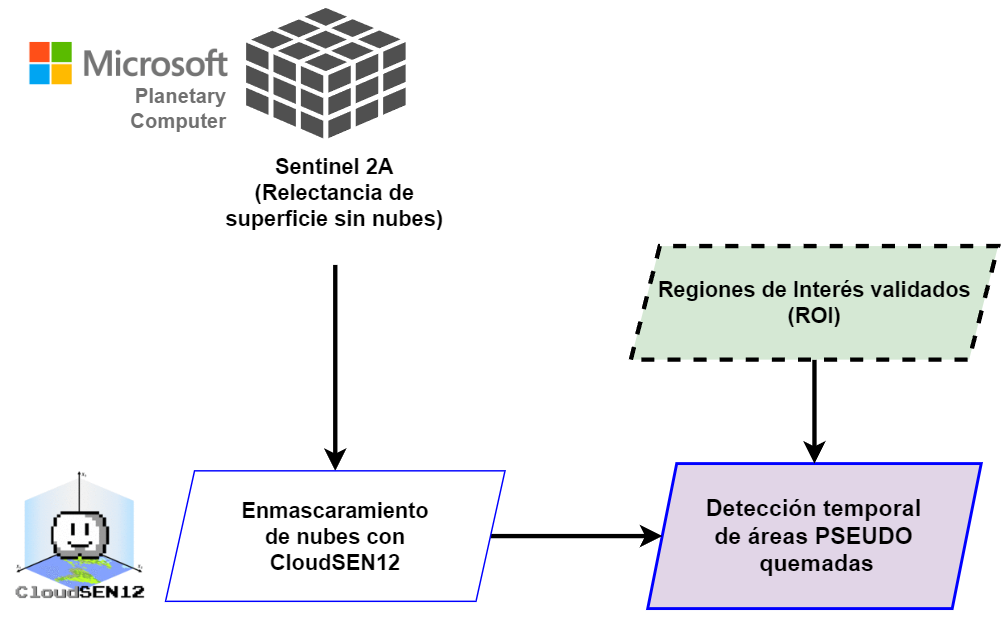
\includegraphics[width=0.6\textwidth]{img/6_metodologia/preprocessimg.png}
    \label{fig:procesamientoimg}
    \begin{flushleft}
        \textit{Nota.} Elaboración propia.        
        \vspace{-\baselineskip}
    \end{flushleft}
\end{figure}

Se filtraron las imágenes históricas de las series temporales, obteniéndose un total de 10,149 imágenes en 74 ROI's de las 79 iniciales.

\subsection{Detección temporal de áreas pseudoquemadas}
Los datos provenientes de Sentinel-2 L2A están disponibles desde el año 2017, lo que implica que cada región de interés (ROI) tiene un máximo aproximado de 400 imágenes disponibles. Esta cantidad considerable de datos dificulta el proceso de selección de imágenes que contengan áreas quemadas, ya que esto requiere una interpretación visual exhaustiva de cada imagen de manera individual.

Para abordar esta dificultad, se emplean métodos basados en reglas para detectar posibles áreas quemadas o pseudoquemas (ver Figura \ref{fig:dBADI}). Esta estrategia permite identificar automáticamente las posibles áreas con quema, facilitando el proceso de identificación y análisis posterior.

\begin{figure}[H]
    \centering
    \caption{Esquema metodológico para la detección pseudoquemas.}
    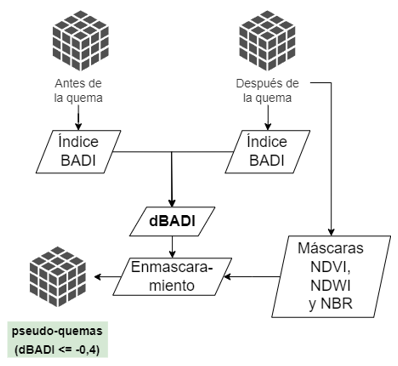
\includegraphics[width=0.5\textwidth]{img/6_metodologia/dBADI.png}
    \label{fig:dBADI}
    \begin{flushleft}
        \textit{Nota.} Elaboración propia.        
        \vspace{-\baselineskip}
    \end{flushleft}
\end{figure}


El cálculo del índice $\Delta BADI$, basado en la propuesta de \citet{farhadi_badi_2023}, se lleva a cabo mediante el procesamiento del BADI utilizando imágenes antes y después del probable evento de quema de la serie temporal en cada ROI. 

Posteriormente, el resultado del umbral $\Delta BADI \leq -0.4$ obtenido se enmascara mediante el uso de $NDVI \leq 0.2$, $NDWI \leq 0$ y $NBR \leq -0.15$ con el objetivo de eliminar áreas 
cubiertas por vegetación, cuerpos de agua y reducir los falsos positivos respectivamente. Esta estrategia detectó quema mayor a una hectárea ($> 1$ ha), equivalente a 100 píxeles de Sentinel-2, en un total de 3,195 imágenes distribuidas en 74 ROI's.

\begin{figure}[H]
    \centering
    \caption{Histograma de áreas pseudoquemadas detectadas (en hectáreas)  en las 74 ROI's.}
    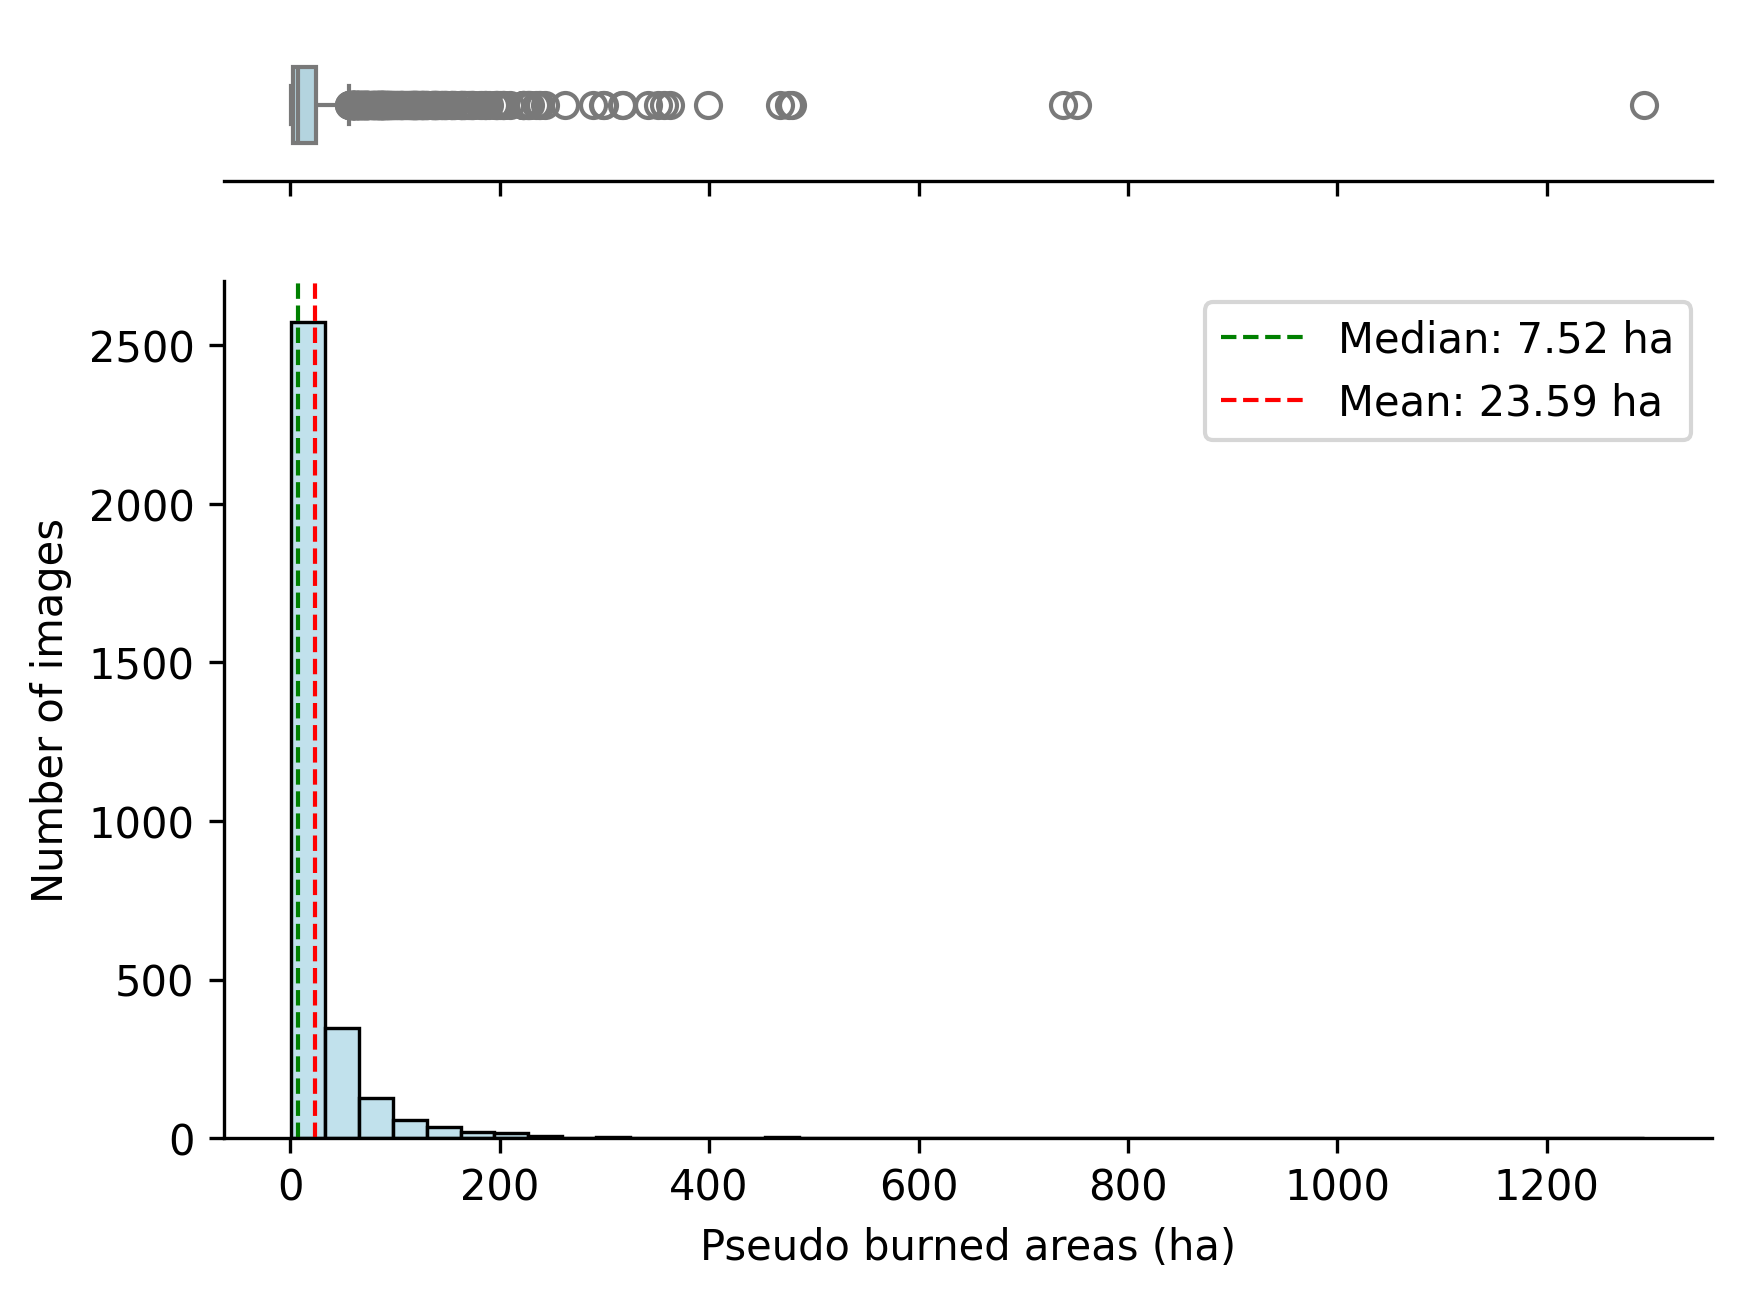
\includegraphics[width=0.7\textwidth]{img/6_metodologia/boxplot_burning.png}
    \label{fig:percentage_burning}
    \begin{flushleft}
        \vspace{-\baselineskip}
        \textit{Nota.} Elaboración propia.        
        \vspace{-\baselineskip}
    \end{flushleft}
\end{figure}

De la Figura \ref{fig:percentage_burning} se observa que la mediana (7.52 ha) y la media (23.59 ha) se encuentran muy cerca del extremo izquierdo del histograma, lo que sugiere una distribución fuertemente sesgada hacia áreas quemadas de menor tamaño. Los outliers, que corresponden a áreas pseudo-quemadas 
significativamente grandes, se localizan en el extremo derecho del histograma y suman un total de 337 imágenes.  

De las 2,858 imágenes restantes, se seleccionan 2,000 mediante un muestreo estratificado, utilizando los percentiles 25, 50 y 75 como criterios para definir los estratos de la distribución 
de áreas quemadas.

\subsection{Selección de imágenes con áreas quemadas}
\label{sec:seleccion_imagenes}
El primer paso para asegurar un alto grado de fiabilidad en la presencia de quema y no quema es a través de la interpretación visual de las imágenes a las cuales se le detectaron pseudoquemas con extensión mayor a 1 hectárea.
Para esta interpretación se utilizan cuatro combinaciones bandas de Sentinel-2 (Tabla \ref{tab:combinaciones}). 

\begin{table}[H]
    \centering
    \caption{Descripción de las combinaciones RGB para diferentes tipos de áreas.}
    \label{tab:combinaciones}
    \begin{tabularx}{\textwidth}{XXX}
        \hline
        \textbf{Nombre} & \textbf{Combinación RGB} & \textbf{Descripción}\\
        \hline
        Color natural & R:B4 - G:B3 - B:B2 & La vegetación sana es verde y las áreas de quema suelen ser de color gris o negro. \\
        Falso Color convencional & R:B8 - G:B4 - B:B3 & La vegetación densa es roja y las áreas de quema suelen ser de color gris o negro. \\
        Infrarrojo de onda corta & R:B8A - G:B12 - B:B4 & La vegetación densa es roja y las áreas de quema suelen ser de color verde. \\
        Agricultura & R:B11 - G:B8 - B:B2 & La vegetación tiene tonos de verde y las áreas de quema suelen ser de color rojizo. \\
        \hline
    \end{tabularx}
    \begin{flushleft}
        \textit{Nota.} Elaboración propia con información de \citet{Sentinel-Hub}        
        \vspace{-\baselineskip}
    \end{flushleft}
\end{table}


Asimismo, se emplean máscaras basadas en índices espectrales, a las cuales se les aplicó una reclasificación binaria utilizando los criterios 
$BADI \geq 0.4$ y $NBR \leq -0.15$. Con estos criterios, se generaron imágenes para identificar áreas quemadas, tal y como se muestra en la Figura \ref{fig:visualizacion} 
que muestra un área típica con la presencia de áreas quemadas.

\begin{figure}[H]
    \centering
    \caption{Combinaciones RGB utilizadas para la selección de imágenes con áreas quemadas.}
    \includegraphics[width=0.55\textwidth]{img/6_metodologia/visualizacion.png}
    \label{fig:visualizacion}
    \begin{flushleft}
        \textit{Nota.} Elaboración propia.        
        \vspace{-\baselineskip}
    \end{flushleft}
\end{figure}

En esta etapa se visualizaron las 2,000 imágenes para verificar la presencia de quema. En promedio, la \textbf{detección temporal de áreas pseudoquemadas} capturó el 52.7\% de las imágenes totales como áreas con quema. 
Es decir 1,054 imágenes en 66 ROI's contenían áreas quemadas y fueron incluidas en el \textbf{etiquetado de imágenes}. 

\subsection{Etiquetado de imágenes}
\label{sec:etiquetado}
Para generar el conjunto de datos se procede a etiquetar manualmente las imágenes utilizando el software IRIS (Figura \ref{fig:iris}) sin la asistencia predictiva por defecto. En este proceso se etiquetan 
las 1,054 imágenes seleccionadas en dos clases: ``quema'' y ``no quema''. Además, se incorpora un \textbf{composite de referencia} como visualización adicional, obtenido a partir de la composición espectral de 25 
imágenes aleatorias de la serie temporal de cada ROI. 

\begin{figure}[H]
    \centering
    \caption{Interfaz de etiquetado en IRIS incoroporando las combinaciones de banda y una imagen de referencia.}
    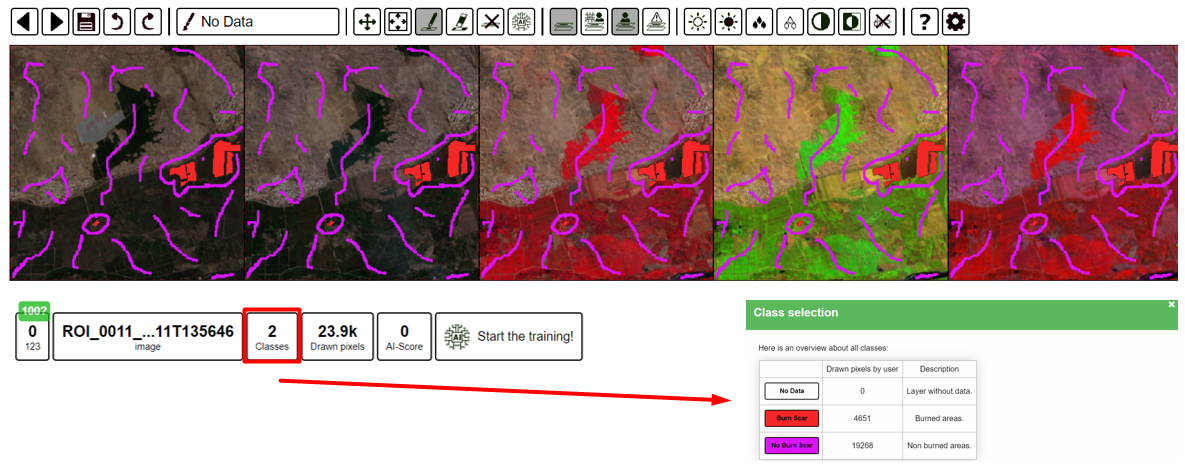
\includegraphics[width=1\textwidth]{img/6_metodologia/iris.png}
    \label{fig:iris}
    \begin{flushleft}
        \vspace{-\baselineskip}
        \textit{Nota.} La visualización es de izquierda a derecha: Composite de referencia (en color natural), Color natural, Falso color convencional, Infrarrojo de onda corta y Agricultura.       
    \end{flushleft}    
\end{figure}

Para realizar esta tarea, se utiliza el método ``Scribble'' (Figura \ref{fig:scribble}), el cual implica etiquetar un pequeño conjunto de muestras en áreas de gran fiabilidad \citep{luo_coarse--fine_2018}. Se obtuvo un 
promedio por imagen de 1,317 píxeles para la clase de ``quema'' y 4,278 píxeles para la clase de ``no quema'', manteniéndose en una proporción que no excedió 
la relación del 5\% y 95\% entre la clase ``quema'' y ``no quema'' respectivamente.

\begin{figure}[H]
    \centering
    \caption{Ejemplo de etiquetado de imágenes utilizando el método ``Scribble''.}
    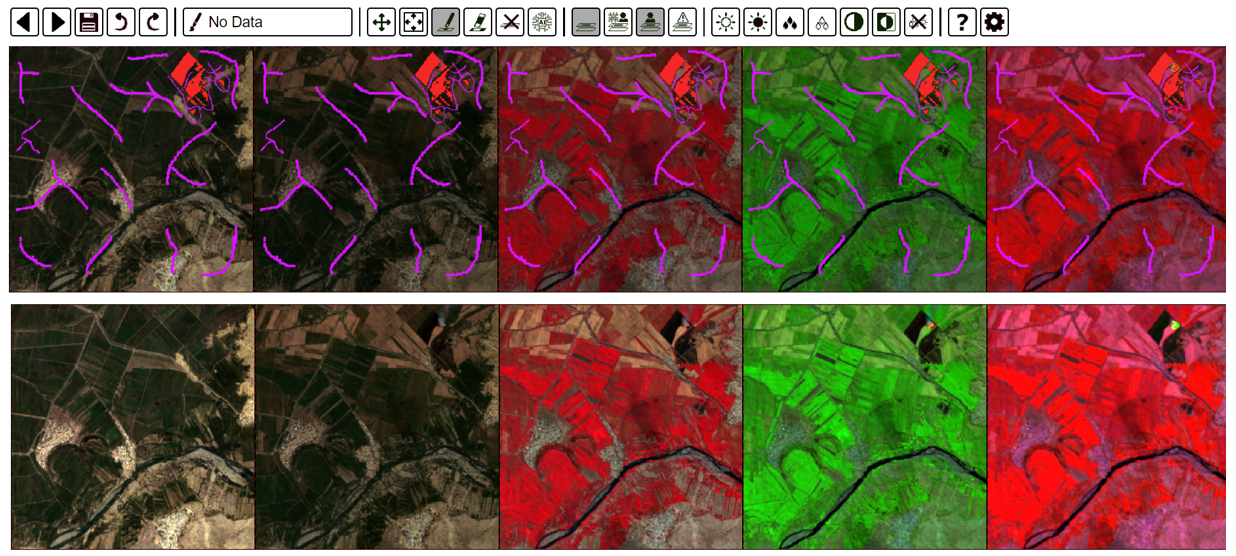
\includegraphics[width=1\textwidth]{img/6_metodologia/scribble.png}
    \label{fig:scribble}
    \begin{flushleft}
        \vspace{-\baselineskip}
        \textit{Nota.} En la parte inferior se muestra la imagen sin etiquetar perteneciente al ROI\_0020\_04, mientras que la parte superior se muestra el resultado del etiquetado con 
        3,715 píxeles clasificados como ``quema'' y 12,225 píxeles clasificados como ``no quema''.       
    \end{flushleft}
\end{figure}

Se considera la diversidad espectral en las áreas etiquetadas, definiendo elementos como cuerpos de agua, suelo desnudo, diferentes tipos de 
vegetación, cultivos inundados, afloramientos rocosos, nubes y áreas artificializadas como ejemplos de ``no quema''.

El protocolo para el etiquetado de la clase ``quema'' se basa en la evaluación visual de las imágenes, respaldada por las características espectrales de una quema en la región del espectro
NIR y SWIR. Para determinar si en una imagen un área es específico corresponde a una quema o no, se establecen un protocolo con cuatro criterios, los cuales se muestran en la Tabla \ref{tab:criterios_quema}. 

Si en una área de la imagen se cumple como mínimo uno de los cuatro criterios establecidos, se etiqueta como ``quema''. Por el contrario, si ninguno de estos criterios se identifica claramente se etiqueta 
como ``no quema''. Esto asegura un alto nivel de confiabilidad en la clasificación visual de las áreas quemadas.

\begin{table}[H]
    \centering
    \caption{Criterios para el protocolo de generación de etiquetas de quema.}
    \label{tab:criterios_quema}
    \begin{tabularx}{\textwidth}{XXX}
        \hline
        \textbf{Criterio} & \textbf{No Quema (0)} & \textbf{Quema (1)} \\
        \hline
        Visualización espectral & Los colores son típicos de otro uso de suelo. & La imagen cumple las tonalidades típicas en las cuatro visualizaciones. \\
        Contraste & El área en cuestión, generalmente extensa, no se diferencia significativamente de sus alrededores. & Hay un contraste evidente con las áreas a su alrededor. \\
        Foco de calor & No se detectan focos de calor en la imagen. & Se detectan focos de calor en la imagen y se aprecia el humo. \\
        Ubicación y contexto espacial & Es difícil determinar si han ocurrido quemas en el área en cuestión. & Está en una ubicación conocida por tener quemas frecuentes. \\
        \hline
    \end{tabularx}
    \begin{flushleft}
        \textit{Nota.} Elaboración propia.        
        \vspace{-\baselineskip}
    \end{flushleft}
\end{table}

En las Figuras \ref{fig:etiquetado1} - \ref{fig:etiquetado4} se presentan ejemplos de imágenes etiquetadas en el software IRIS según los principales criterios establecidos, en donde las áreas 
clasificadas como ``quema'' se muestran en rojo y las áreas clasificadas como ``no quema'' se muestran en morado.

\begin{figure}[H]
    \centering
    \caption{Visualización en IRIS según el criterio de visualización espectral para una imagen en la ROI\_0097\_04.}
    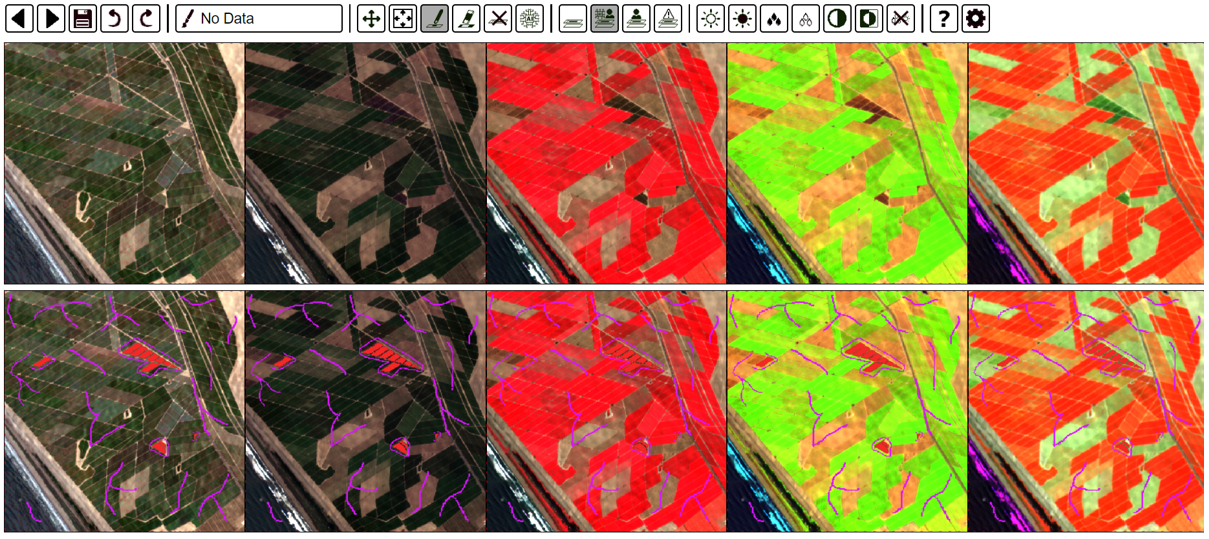
\includegraphics[width=1\textwidth]{img/6_metodologia/etiquetado_1.png}
    \label{fig:etiquetado1}
    \begin{flushleft}
        \vspace{-\baselineskip}
        \textit{Nota.} En la parte superior se muestra la imagen sin etiqueta, mientras que en la parte inferior se presenta la imagen con las etiquetas aplicadas. Elaboración propia.        
        \vspace{-\baselineskip}
    \end{flushleft}
\end{figure}

\begin{figure}[H]
    \centering
    \caption{Visualización en IRIS según el criterio de contraste para una imagen en la ROI\_0020\_01.}
    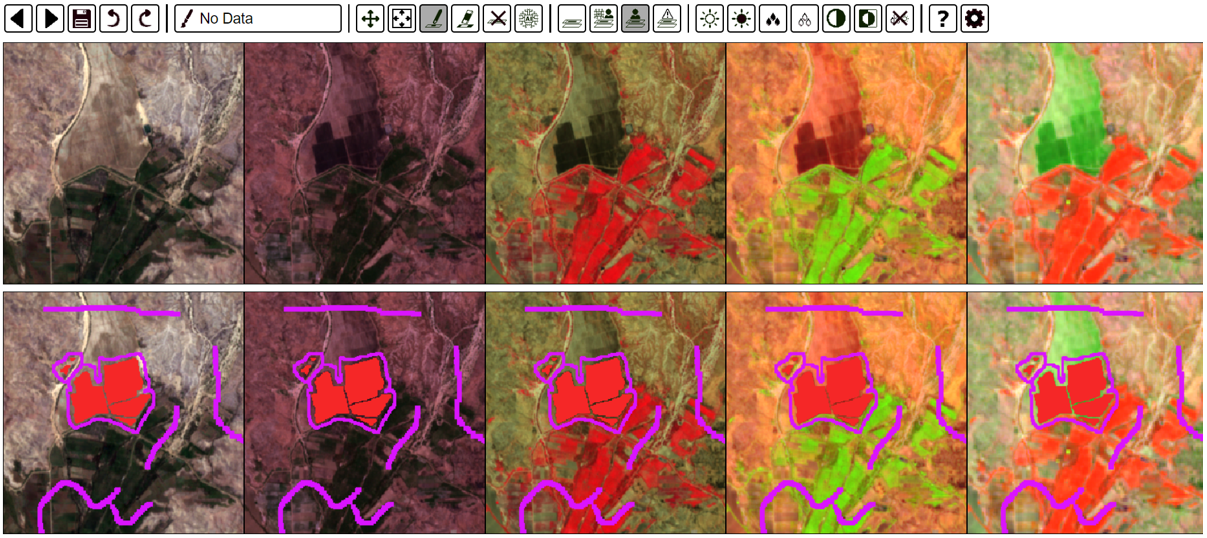
\includegraphics[width=1\textwidth]{img/6_metodologia/etiquetado_2.png}
    \label{fig:etiquetado2}
    \begin{flushleft}
        \vspace{-\baselineskip}
        \textit{Nota.} En la parte superior se muestra la imagen sin etiqueta, mientras que en la parte inferior se presenta la imagen con las etiquetas aplicadas. Elaboración propia.        
        \vspace{-\baselineskip}
    \end{flushleft}
\end{figure}

\begin{figure}[H]
    \centering
    \caption{Visualización en IRIS según el criterio de foco de calor para una imagen en la ROI\_0084\_01.}
    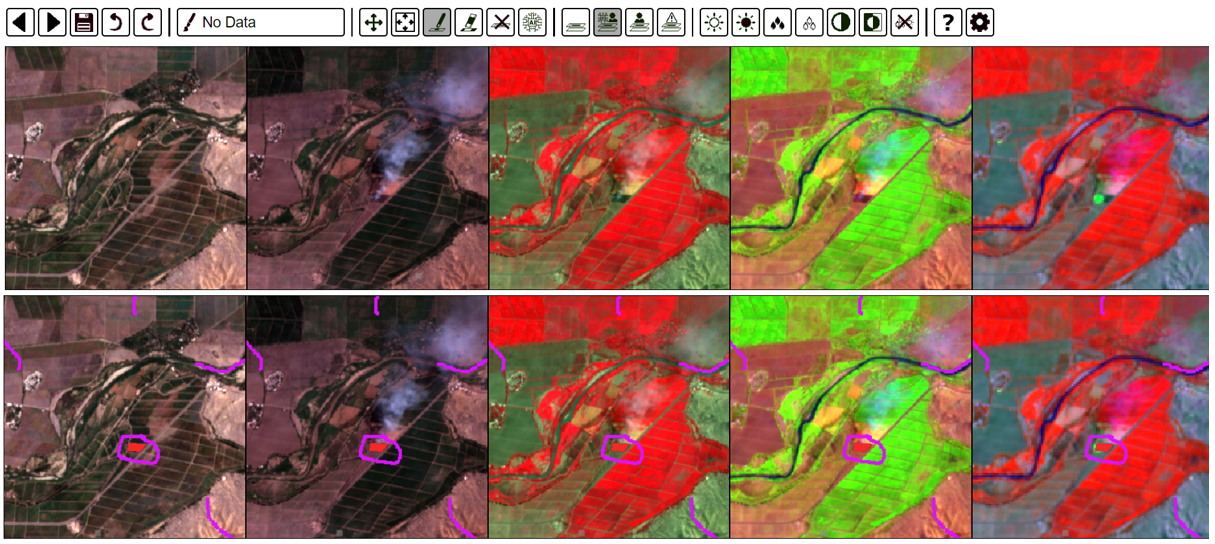
\includegraphics[width=1\textwidth]{img/6_metodologia/etiquetado_3.png}
    \label{fig:etiquetado3}
    \begin{flushleft}
        \vspace{-\baselineskip}
        \textit{Nota.} En la parte superior se muestra la imagen sin etiqueta, mientras que en la parte inferior se presenta la imagen con las etiquetas aplicadas. Elaboración propia.        
        \vspace{-\baselineskip}
    \end{flushleft}
\end{figure}

\begin{figure}[H]
    \centering
    \caption{Visualización en IRIS según el criterio de ubicación y contexto espacial para una imagen en la ROI\_0011\_01.}    
    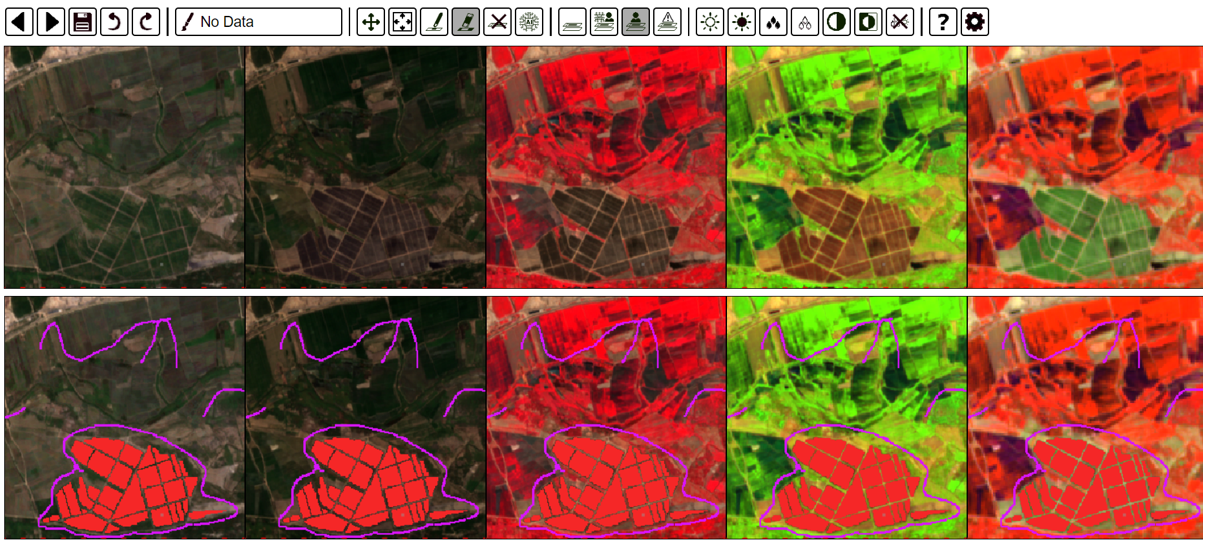
\includegraphics[width=1\textwidth]{img/6_metodologia/etiquetado_4.png}
    \label{fig:etiquetado4}
    \begin{flushleft}
        \vspace{-\baselineskip}
        \textit{Nota.} En la parte superior se muestra la imagen sin etiqueta, mientras que en la parte inferior se presenta la imagen con las etiquetas aplicadas. Elaboración propia.        
        \vspace{-\baselineskip}
    \end{flushleft}
\end{figure}

En ciertos casos, se ha decidido establecer manualmente un umbral, especialmente cuando la quema exhibe tonalidades sutiles que no son consideradas 
significativas o relevantes.

\begin{figure}[H]
    \centering
    \caption{Visualización en IRIS según el criterio de delimitación de umbral para una imagen en la ROI\_0094\_02.}
    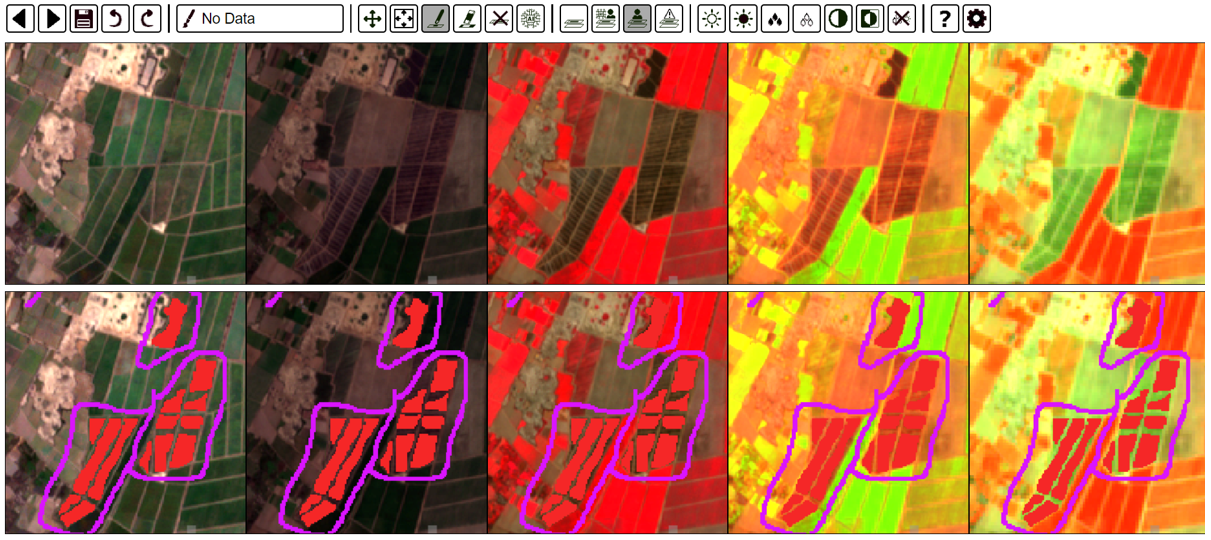
\includegraphics[width=1\textwidth]{img/6_metodologia/etiquetado_5.png}
    \label{fig:etiquetado5}
    \begin{flushleft}
        \vspace{- \baselineskip}
        \textit{Nota.} En la parte superior se muestra la imagen sin etiqueta, mientras que en la parte inferior se presenta la imagen con las etiquetas aplicadas. Elaboración propia.        
        \vspace{-\baselineskip}
    \end{flushleft}
\end{figure}

\subsection{Generación del conjunto de datos para la detección de quemas}

Una vez etiquetadas las imágenes, se procede a la generación de un conjunto de datos de entrenamiento para los modelos. Este conjunto de datos se compone de 1,054 imágenes de 
$512 \times 512$ píxeles con una profundidad de 16 bandas.

Estas 16 bandas comprenden el apilamiento de las 10 bandas de Sentinel-2, que abarcan las bandas del espectro visible (B02, B03, B04), el borde rojo (B05, B06, B07, B8A), el infrarrojo cercano (B8) y el
infrarrojo de onda corta (B11, B12). Además, se incluyen índices específicos como los de quema (NBR y BADI), vegetación (NDVI), agua (NDWI), así como variables topográficas como la pendiente (en \%) y la distancia 
a la cobertura agrícola (en metros). Siendo estas dos últimas variables definidas a continuación:

\subsubsection{Pendiente.}
La pendiente es una variable topográfica que se calcula a partir de un modelo digital de elevación (DEM) y se utiliza para caracterizar la inclinación del terreno. En este estudio, se utilizó el 
producto \href{https://planetarycomputer.microsoft.com/dataset/nasadem}{NASA DEM}, que ofrece datos topográficos globales con una resolución horizontal de 1 segundo de arco (30 m) y 
se derivan principalmente de los capturados durante la Shuttle Radar Topography Mission (SRTM).

La relevancia de la pendiente en la detección de la quema de caña de azúcar radica en que las áreas de menor pendiente son más aptas para el cultivo de este tipo de cosecha. Además, la pendiente permite diferenciar 
los suelos desnudos ubicados en los valles costeros con alta inclinación.

\subsubsection{Distancia a la cobertura agrícola.}
La distancia a la cobertura agrícola es una variable utilizada para medir la proximidad de un píxel a áreas de cultivo. Esta variable se calculó utilizando el mapa de 
\href{https://planetarycomputer.microsoft.com/dataset/io-lulc-annual-v02}{ESRI Land Use}, que tiene una resolución de 10 metros.

Este conjunto de datos consiste en una serie temporal de mapas globales anuales de uso y cobertura del suelo (LULC) desde 2017 hasta 2023. Los mapas se derivan de imágenes Sentinel-2 de la ESA y 
proporcionan predicciones de LULC para 9 clases a lo largo del año, ofreciendo una representación precisa y representativa de cada año.

Su relación con la detección de quema de caña de azúcar se explica en que valores bajos de distancia a la cobertura agrícola indican áreas cercanas a cultivos. Esta variable es crucial para identificar las zonas 
que están directamente involucradas en actividades agrícolas y, por ende, potencialmente sujetas a quemas de caña de azúcar.

\subsection{Implementación del modelo CNN}
Se implementa una red neuronal convolucional con una arquitectura U-Net y un codificador \textbf{ResNet50} \citep{al_dabbagh_2023}, preentrenado en el conjunto de datos ImageNet. 
En la Figura \ref{fig:unet_architecture} muestra la arquitectura de la red U-Net, que toma como entrada una imagen con dimensiones de $512 \times 512 \times 16$ (profundidad de 16 bandas), 
y genera un mapa de segmentación de dimensiones $512 \times 512 \times 1$ que representa la probabilidad de quema en cada píxel. 

\begin{figure}[H]
    \centering
    \caption{Arquitectura U-Net para la segmentación semántica.}
    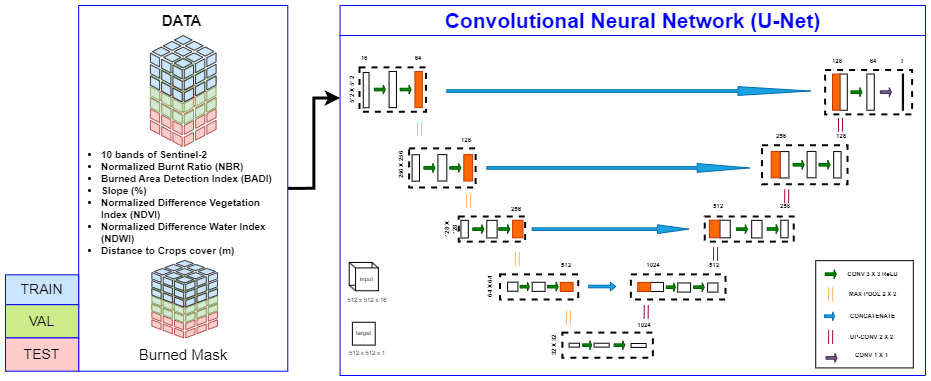
\includegraphics[width=1\textwidth]{img/6_metodologia/unet.png}
    \label{fig:unet_architecture}
    \begin{flushleft}
        \vspace{-\baselineskip}
        \textit{Nota.} Elaboración propia.        
        \vspace{-\baselineskip}
    \end{flushleft}
\end{figure}

\subsection{Implementación del Gradient Boosting Decision Tree}
Se propone el modelo de Gradient Boost Decision Tree, implementado  en el framework de LightGBM en Python, para generar predicciones. El modelo se entrena con un conjunto de datos estructurado en forma tabular, donde cada fila corresponde a 
un pixel y cada columna a una de las 17 bandas disponibles, incluyendo la etiqueta correspondiente.

Para prevenir el sobreajuste y asegurar una evaluación más precisa y confiable del rendimiento del modelo, se emplea la validación cruzada de 10 particiones o pliegues (ten-fold cross-validation). En este enfoque, el conjunto de datos se divide en 
10 partes iguales; el modelo se entrena con 9 partes y se evalúa con la parte restante. 

Este proceso se repite en 10 iteraciones, de modo que, en cada iteración, una parte diferente actúa como conjunto de validación mientras las restantes se utilizan 
para el entrenamiento. (Figura \ref{fig:crossval}).

\begin{figure}[H]
    \centering
    \caption{Esquema de la validación cruzada en diez pliegues.}
    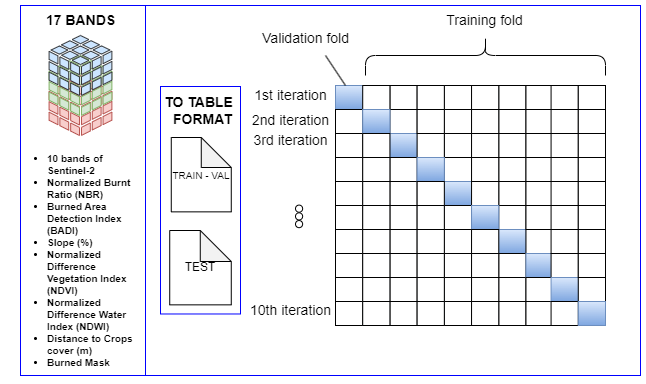
\includegraphics[width=0.7\textwidth]{img/6_metodologia/crossval.png}  
    \label{fig:crossval}
    \begin{flushleft}
        \vspace{-\baselineskip}
        \textit{Nota.} Elaboración propia.        
        \vspace{-\baselineskip}
    \end{flushleft}
\end{figure}

La aplicación del validación cruzada de pliegues permitió obtener diez modelos utilizando LightGBM (Figura \ref{fig:lightgbm}); se eligió el menor valor de probabilidad en cada píxel como medida de consenso entre los modelos
debido que las etiquetas se crearon en áreas de alta fiabilidad, donde generalmente todos los modelos coinciden en clasificar el píxel como ``quema''. 
 \begin{figure}[H]
    \centering
    \caption{Modelo LightGBM para cada pliegue en la validación cruzada.}
    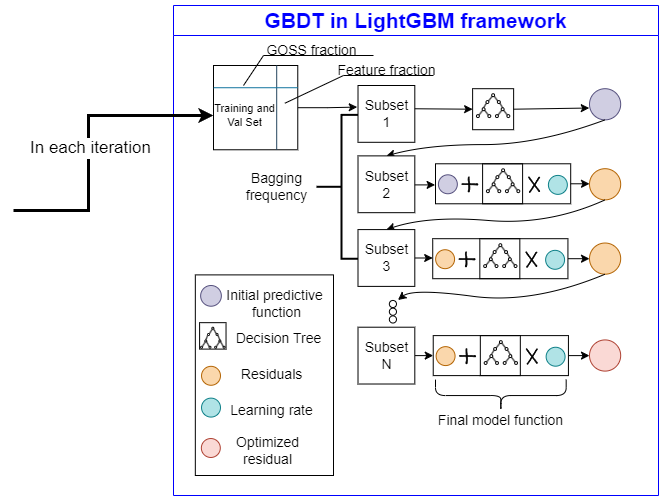
\includegraphics[width=0.7\textwidth]{img/6_metodologia/gbdt.png}  
    \label{fig:lightgbm}
    \begin{flushleft}
        \vspace{-\baselineskip}
        \textit{Nota.} Elaboración propia.        
        \vspace{-\baselineskip}
    \end{flushleft}
 \end{figure}

\subsection{Implementación del modelo Stacking}
El modelo ensamblado de stacking utiliza como conjunto de datos los mapas de probabilidad generados por los dos modelos previos: U-Net y GBDT (Gradient Boosting Decision Tree). 

A partir de estos mapas de probabilidad, se entrena un metamodelo de regresión logística cuyo propósito es combinar las predicciones de ambos modelos base para generar un mapa de probabilidades final que integra 
la información de ambos enfoques. 

Una vez obtenido el mapa de probabilidades final del modelo Stacking, se procede a convertir en una máscara binaria. Para esto, se define un umbral óptimo basado en la curva ROC, seleccionando el 
punto que maximiza el equilibrio entre la sensibilidad (Precision) y la especificidad (Recall). 

\begin{figure}[H]
    \centering
    \caption{Esquema del modelo de ensamblado de stacking.}
    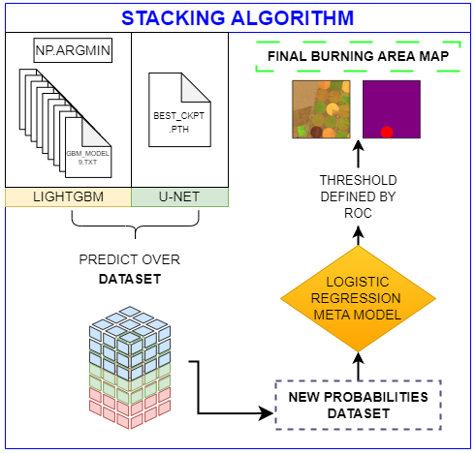
\includegraphics[width=0.6\textwidth]{img/6_metodologia/stacking.png}  
    \label{fig:stacking}
    \begin{flushleft}
        \vspace{-\baselineskip}
        \textit{Nota.} Elaboración propia.        
        \vspace{-\baselineskip}
    \end{flushleft}
 \end{figure}

\subsection{Validación del umbral de clasificación para el modelo Stacking} 
\label{sec:ajuste_umbral}

La validación del umbral de clasificación definido anteriormente debe de verificarse visualmente en un conjunto de imágenes de validación.
Estas imágenes de validación corresponden a áreas quemadas que son coherentes con los 471 reportes dentro del registro histórico de la OEFA.

Para este fin, de un total de 478 imágenes analizadas se obtuvieron 58 imágenes que cumplían con los siguientes criterios:
\begin{itemize} 
    \item La imagen muestra una extensión de quema dentro de un rango de \pm 7 días respecto a la fecha reportada al OEFA. 
    \item La imagen muestra una extensión de quema que es visualmente detectable. 
    \item Las coordenadas del evento de quema son espacialmente coherentes con la ubicación mostrada en la imagen. 
\end{itemize}

Este proceso asegura que el umbral de clasificación se corresponda con la realidad de las áreas quemadas, garantizando que el modelo Stacking sea capaz de detectar de manera precisa y confiable las áreas 
quemadas en las imágenes de Sentinel-2 con el umbral de clasificación definido.

\subsection{Inferencia del modelo Stacking en un área piloto}
\label{sec:inferencia}
Tras validar el umbral de clasificación, se procede a realizar la inferencia en el distrito de Laredo (área piloto), ubicado en el departamento de La Libertad, uno de los doce distritos de la provincia de Trujillo, centrando el análisis en un período reciente 
de enero de 2023 a agosto de 2024. 

Este distrito, con una población proyectada en 2022 de 44,440 habitantes según datos del 
\citet{inei_peru_2022}, fue elegido debido a su proximidad a los fundos azucareros propiedad del ingenio azucarero Laredo S.A.A. 

Esta empresa carece de un instrumento de gestión ambiental actualizado que incluya la cosecha verde y un cronograma más detallado 
para el manejo de quemas (ver Figura \ref{fig:laredo_programa}), ya que su último Plan de Adecuación y Manejo Ambiental (PAMA) data de 2004 (Rg.G. N° 002-2004-INRENA-OGATEIRN).

\begin{figure}[H]
    \centering
    \caption{Cronograma de actividades para la implementa de medidas de mitigación en el PAMA de Laredo S.A.A.}
    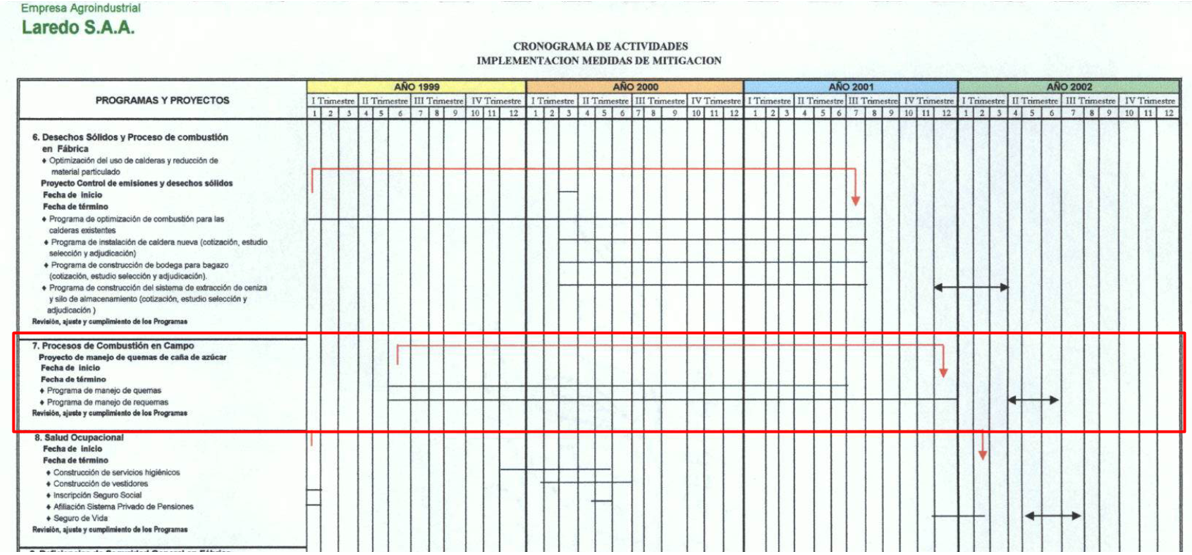
\includegraphics[width=1\textwidth]{img/6_metodologia/laredo_programa.png}  
    \label{fig:laredo_programa}
    \begin{flushleft}
        \vspace{-\baselineskip}
        \textit{Nota.} En la parte seleccionada de rojo, se observa que el PAMA de Laredo S.A.A. solo contempla este programa ante la quema de caña de azúcar. Extraído de \citet[p. 24]{laredo_saa_programa_2000}        
        \vspace{-\baselineskip}
    \end{flushleft}
 \end{figure}

El criterio de selección es el mismo de la Sección \ref{sec:seleccion_imagenes}, partiendo de la selección de la cobertura de nubosidad menor al 10\% y la detección de áreas pseudoquemadas. 
De esta selección se obtuvieron 30 imágenes de Sentinel-2 L2A para el 
área piloto de Laredo (Figura \ref{fig:laredo}). 

\begin{figure}[H] 
    \centering 
    \caption{Área piloto seleccionada para la inferencia del modelo.} 
    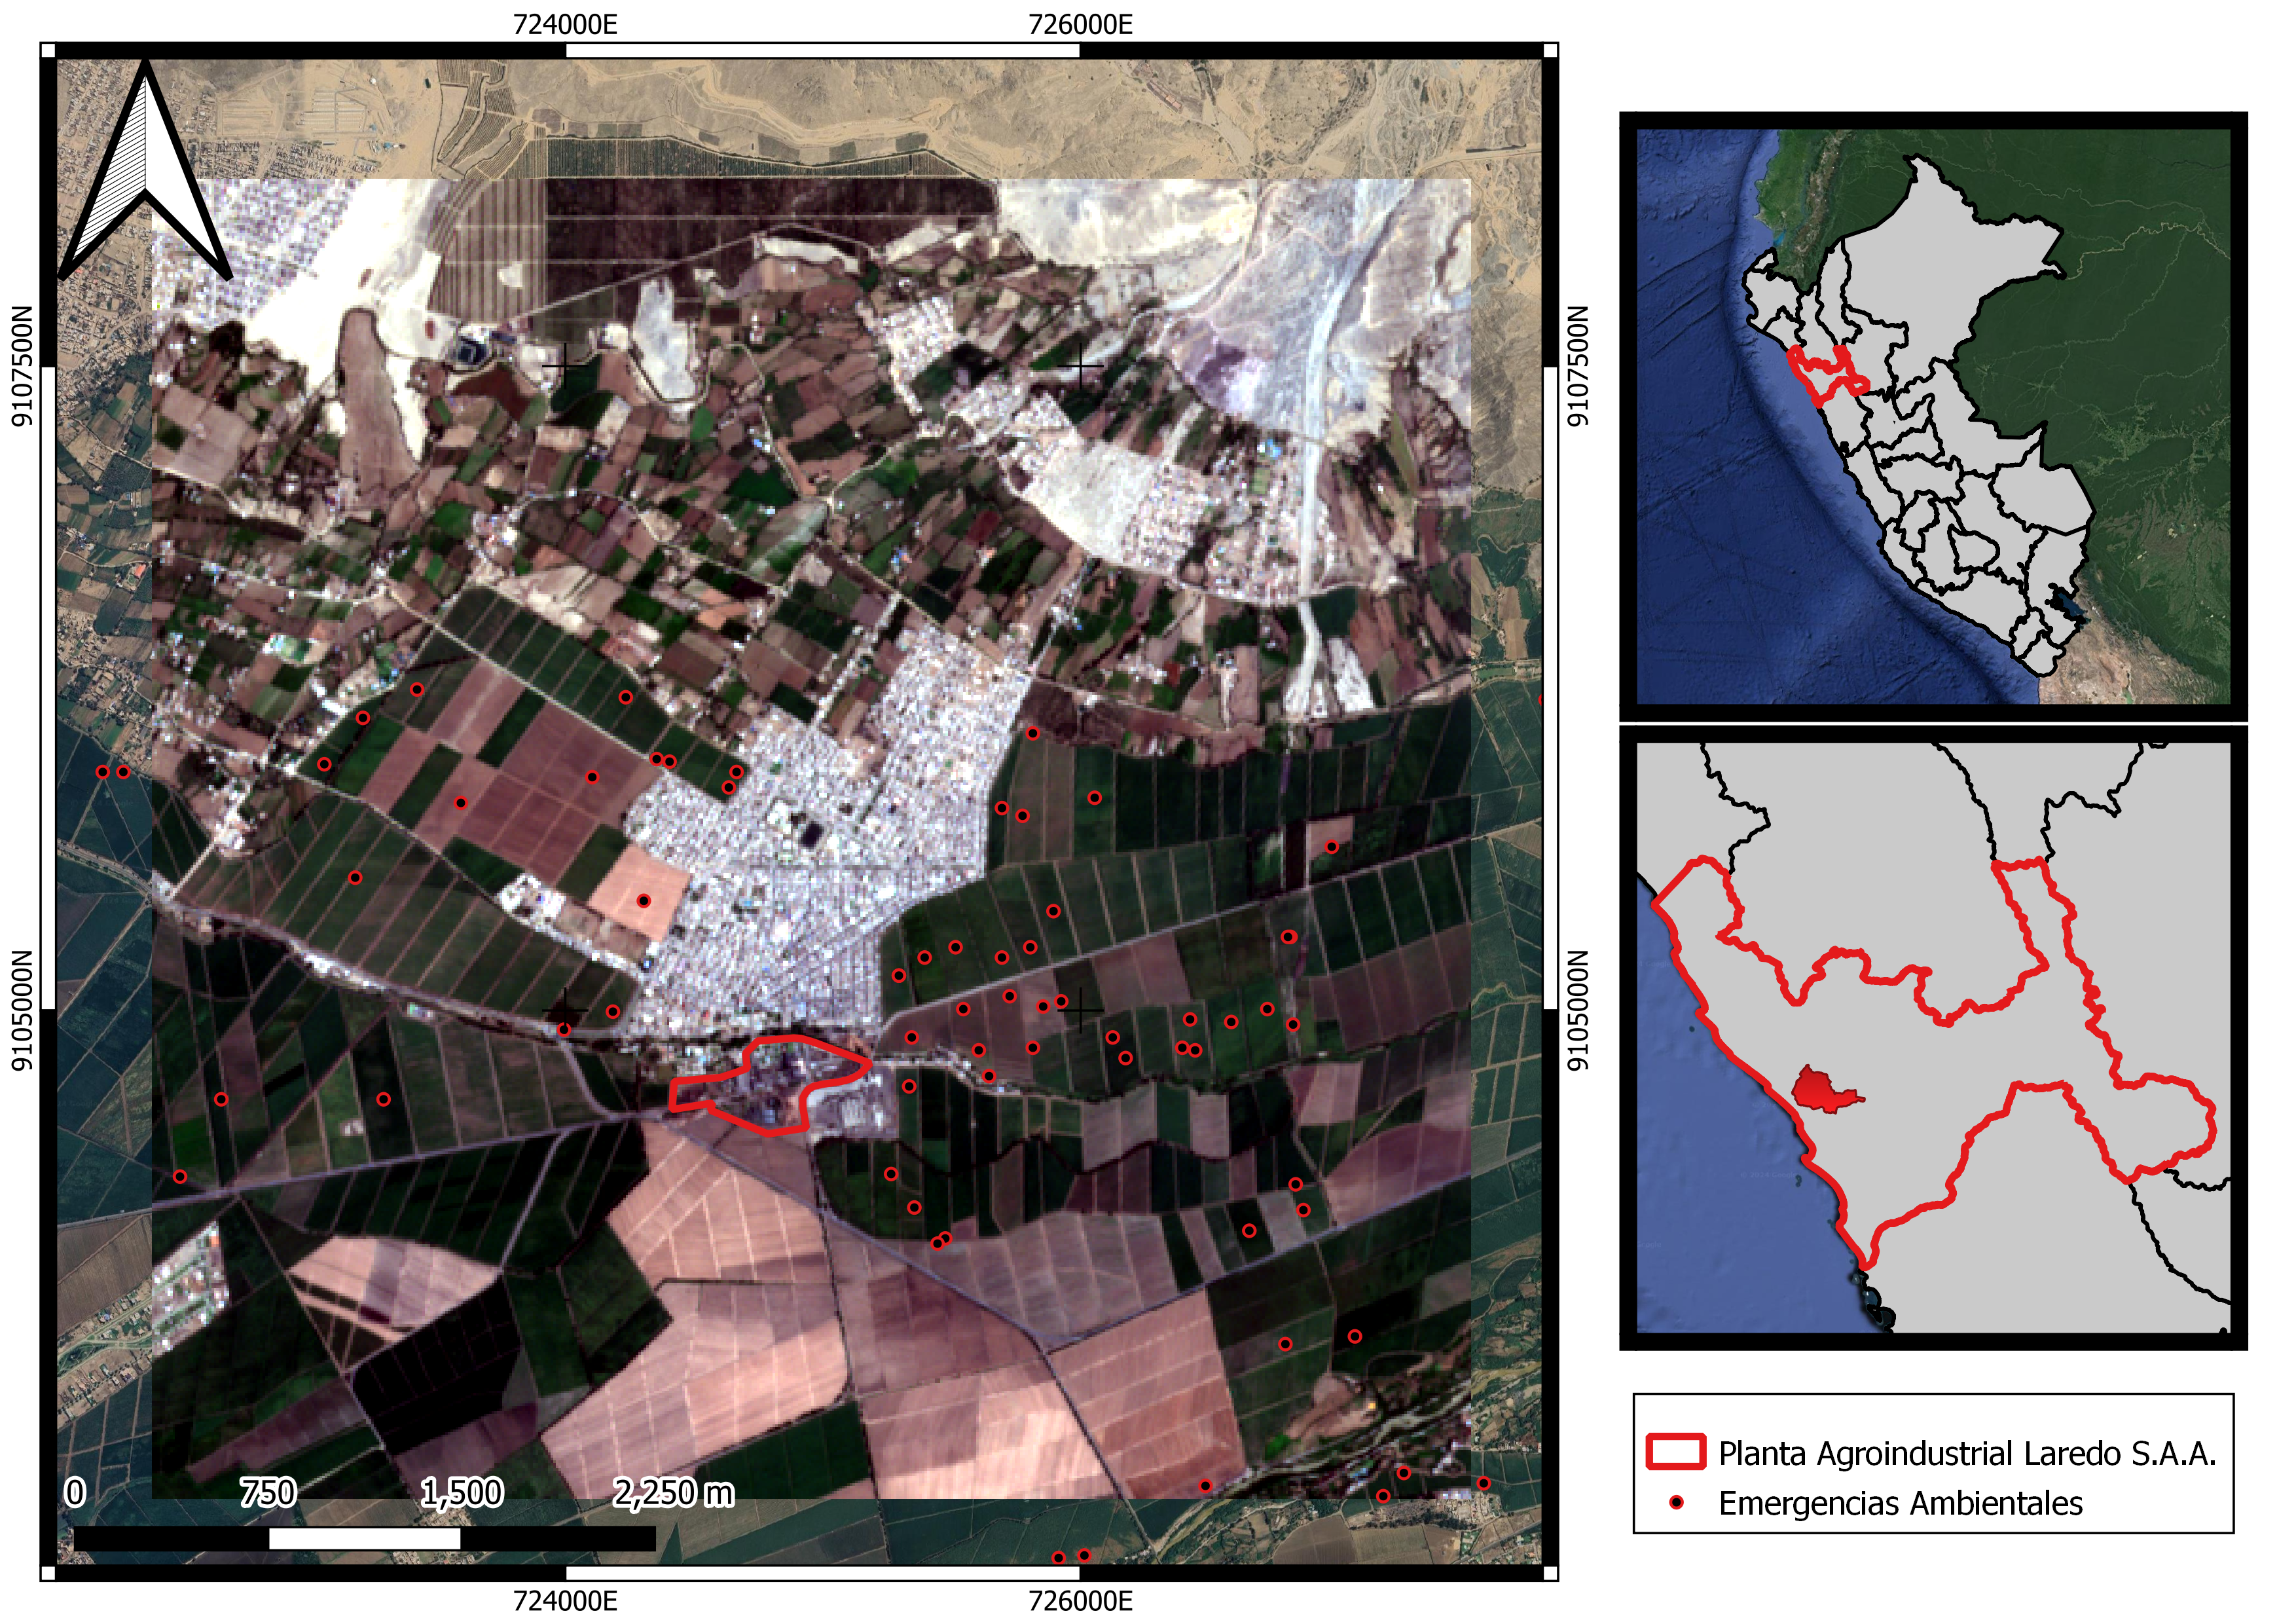
\includegraphics[width=0.9\textwidth]{img/6_metodologia/laredo.png}
    \label{fig:laredo} 
    \begin{flushleft} 
        \vspace{-\baselineskip} 
        \textit{Nota.} Elaboración propia.
        \vspace{-\baselineskip} 
    \end{flushleft} 
\end{figure}




